%=======================================================================
%  Briefings in Bioinformatics -- Problem-solving Protocol
%  Official OUP class: oup-authoring-template (contemporary, numbered refs)
%
%  "How should genomic foundation models be evaluated for metagenomic
%   taxonomic classification?"
%
%  Compiles with pdflatex + bibtex on any full TeX Live / Overleaf.
%  The OUP class + .bst files are bundled in this repo, so no extra
%  installation is required.  Build order:  pdflatex -> bibtex -> pdflatex x2
%  (or: latexmk -pdf main.tex).
%=======================================================================
\documentclass[unnumsec,webpdf,contemporary,large,numbered]{oup-authoring-template}

% --- extra packages not already provided by the class ---
% (class already loads: graphicx, caption, amsmath, amssymb, array, xcolor,
%  natbib, multirow, url, hyperref, tikz)
% NB: tables use the class's tabular*/\toprule/\botrule house style, not
% tabularx (tabularx is incompatible with the class's rule macros).
\usetikzlibrary{arrows.meta,positioning,fit}

% Enable natbib sort&compress so multi-citations render as [8-14], not
% [8, 9, 10, 11, 12, 13, 14]. (The class loads natbib itself, so we set the
% switches directly rather than via a package option.)
\makeatletter
\def\NAT@sort{\@ne}\def\NAT@cmprs{\@ne}
\makeatother

\graphicspath{{figures/}}

% The OUP class defaults the running-head society logo to a PNAS Nexus image
% that is not shipped with the bundle; blank it out (documented in the class).
\def\societylogo{}

% colour used by the Figure 1 schematic
\definecolor{bibblue}{RGB}{0,63,114}

% For peer review you may enable line numbers (uncomment):
%\usepackage[mathlines,switch]{lineno}\linenumbers

\begin{document}

\journaltitle{Briefings in Bioinformatics}
\DOI{}
\copyrightyear{2026}
\pubyear{2026}
\access{Advance Access Publication Date: Day Month Year}
\appnotes{Problem-solving Protocol}

\firstpage{1}

\title[GFMs for metagenomic taxonomic classification]{How should genomic
foundation models be evaluated for metagenomic taxonomic classification?
A controlled benchmark of pre-training, tokenization, and data scaling}

\author[1,$\ast$]{Ming-Ju Yang\ORCID{0000-0000-0000-0000}}
\author[1]{Second Author}

\address[1]{\orgdiv{Graduate Institute of Biomedical Electronics and
Bioinformatics}, \orgname{National Taiwan University},
\orgaddress{\state{Taipei}, \country{Taiwan}}}

\corresp[$\ast$]{Corresponding author. \href{mailto:r13945009@ntu.edu.tw}{r13945009@ntu.edu.tw}}

%\received{Date}{0}{Year}
%\revised{Date}{0}{Year}
%\accepted{Date}{0}{Year}

\abstract{\textbf{Background:} Genomic foundation models (GFMs) have shown
promise across many genomic tasks, yet their utility for metagenomic
short-read taxonomic classification---where reads are $\sim$150\,bp and
per-read taxonomic signal is sparse---remains poorly characterized, and it is
unclear which design axis (pre-training, tokenization, or data scale) actually
governs performance.
\textbf{Methods:} We present a controlled benchmark that varies one factor at a
time while holding architecture, data, and evaluation constant. Using reads
simulated from a unified human-gut genome catalogue across 120 genera and
1{,}535 species, we ablate data scale (500K--250M reads), pre-training
(a 498M-parameter pre-trained backbone versus a randomly initialized one),
tokenization (6/12/13-mer, overlapping versus non-overlapping), and evaluation
protocol (read-level accuracy, sample-level abundance estimation, and binary
detection), and compare against the alignment-free classifier Kraken\,2.
\textbf{Results:} Tokenization, not backbone pre-training, sets the ceiling:
within one architecture (MetaTransformer, from scratch), changing a 6-mer
tokenizer to an overlapping 13-mer raises genus Top-1 from 48.9\% to 87.4\% and
keeps scaling to 98.7\% at 250M, whereas 6-mer models saturate ($+0.22$ pp) and
cannot even \emph{fit} their training set beyond $\sim$66\%---a representational,
not optimization, ceiling. At matched 6-mer a pre-trained backbone helps
(67.1\% versus 47.0\%), but its tokenizer is fixed at 6-mer, so the ceiling
resists more pre-training or data. At the sample level a 67\%-accurate model
reaches Pearson $r=0.99$ for genus abundance, but a properly configured
Kraken\,2$+$Bracken pipeline matches it ($r=0.997$) and detects better; the
distinct value of GFMs is read-level accuracy and behaviour outside the reference
database, not abundance. On real mock-community data all methods fall to
$r\approx0.4$--$0.6$ with no clear winner, exposing a large closed-set-to-real
gap.
\textbf{Conclusion:} Tokenization design is the critical, and currently
under-appreciated, factor for GFM-based metagenomic classification. We translate
these findings into use-case-specific recommendations and argue that future
microbial foundation models should be pre-trained with overlapping long-$k$
tokenization.}

\keywords{genomic foundation models, metagenomics, taxonomic classification,
tokenization, benchmarking, short-read sequencing}

\boxedtext{Key Points}{
\begin{itemize}
\item Data scaling is tokenizer-dependent: increasing training data from 50M to
250M reads yields almost no gain for a non-overlapping 6-mer model
($+0.22$ percentage points) but an 11-point gain for an overlapping 13-mer model
($87.4\%\!\rightarrow\!98.7\%$).
\item Tokenization, not backbone pre-training, sets the performance ceiling:
within one architecture, changing a 6-mer tokenizer to an overlapping 13-mer
lifts genus Top-1 from 48.9\% to 87.4\%---a larger effect than pre-training, and
one NT-v2 cannot access because its tokenizer is fixed at 6-mer.
\item At matched 6-mer tokenization a pre-trained backbone still helps (NT-v2
67.1\% versus 47.0\% for a from-scratch model), so pre-training and tokenization
are separable and both matter.
\item Read-level accuracy and sample-level utility diverge: a 67\%-accurate read
classifier reaches Pearson $r=0.99$ for genus abundance on simulated
in-database samples, but that ranking does not transfer to a real mock
community (two D6331 replicates: $r\approx0.4$--$0.6$ for all methods, including
Kraken\,2$+$Bracken, with overlapping uncertainty at $n{=}11$ genera).
\item We give practical, use-case-specific recommendations and argue that future
microbial foundation models should be pre-trained with overlapping long-$k$
tokenization.
\end{itemize}}

\maketitle

\section{Introduction}
\label{sec:intro}

Metagenomic taxonomic classification---assigning each sequencing read to the
organism it originated from---is a foundational step in microbiome analysis,
underpinning studies of community composition, host--microbe interaction, and
clinical diagnostics \citep{Quince2017,HMP2012}. The dominant production tools
are alignment-free $k$-mer methods such as Kraken\,2 and Centrifuge, which match
long exact $k$-mers ($k\approx 31$--$35$) against a reference database and are
fast, accurate, and interpretable when the target organism is well represented
in that database \citep{Wood2019,Kim2016}. Their weaknesses are equally
well established: performance degrades sharply on organisms absent from or
poorly covered by the reference, and exact-match indexing cannot exploit the
distributional structure of sequence that a learned model can
\citep{Ye2019,Breitwieser2019,McIntyre2017}.

In parallel, genomic foundation models (GFMs)---large self-supervised
transformers pre-trained on genomic sequence---have advanced rapidly, with
Nucleotide Transformer, DNABERT/DNABERT-2, HyenaDNA, Caduceus, and Evo
demonstrating strong transfer to regulatory, variant-effect, and
genome-design tasks \citep{DallaTorre2023,Ji2021,Zhou2024dnabert2,
Nguyen2023hyena,Schiff2024caduceus,Nguyen2024,Brixi2025}. This success invites
an obvious question for the microbiome community: \emph{can, and should, GFMs be
used for metagenomic short-read taxonomic classification?} The setting is
adversarial for a foundation model. Reads are short ($\sim$150\,bp), the
taxonomic signal per read is faint, the label space is large and
long-tailed, and most GFMs were pre-trained on eukaryotic (often
human) genomes rather than the bacterial and archaeal diversity that
dominates real communities. Prior neural approaches such as DeepMicrobes,
BERTax, and MetaTransformer show that learned read classifiers are feasible
\citep{Liang2020,Mock2022bertax,Wichmann2023}, but they do not isolate
\emph{why} they work, and they predate the current generation of large
pre-trained backbones. More recently, ICCTax adapted the HyenaDNA genomic
language model to hierarchical taxonomic classification with an explicit focus on
out-of-distribution generalization \citep{Gao2025icctax}. Our focus is
complementary rather than competing: ICCTax classifies kilobase-scale contigs
(1{,}500\,bp) with a single purpose-built classifier, whereas we evaluate
150\,bp shotgun reads, benchmark several transformer GFMs rather than proposing
one model, and isolate whether pre-training, tokenization, or data scale
controls performance.

The practical decision facing a method developer is therefore not ``does a
GFM work at all'' but ``which design choice actually matters''. A GFM-based
classifier is defined by at least four largely independent axes: (i) how much
data it is trained on; (ii) whether the backbone is pre-trained or trained
from scratch; (iii) how the sequence is tokenized (the $k$-mer length and
whether tokens overlap); and (iv) the level at which the output is
evaluated---per read, or aggregated to a sample-level community profile.
These axes are usually entangled in published comparisons, so a reader cannot
tell whether a reported gain comes from a bigger model, more data, or a
different tokenizer. A recent study of tokenizer choice in genomic language
models \citep{Lindsey2025tokenizer} underscores that this axis alone can
dominate, but its effect has not been quantified against pre-training and data
scale in the metagenomic read-classification setting.

This paper answers the methodological question head-on with a controlled
benchmark that changes \emph{one factor at a time}. Holding architecture,
training data, and evaluation protocol fixed, we separately measure the effect
of data scale, pre-training, and tokenization, and we evaluate both at the
read level and at the sample level against Kraken\,2 (raw and with Bracken
re-estimation), with a preliminary real mock-community check. Our central finding is
that the axis most often left unexamined---tokenization---is the one that sets
the performance ceiling, while data scaling helps only until that ceiling is
reached and pre-training contributes a smaller but real gain once tokenization
is fixed. We then translate these findings into concrete, use-case-specific
recommendations for practitioners and for the design of the next generation of
microbial foundation models. Sections are organized as a problem-solving
protocol: we first explain why the task is hard
(Section~\ref{sec:challenges}), describe a leakage-controlled benchmark and a
dual read/sample evaluation (Section~\ref{sec:design}), then present the data
scaling (Section~\ref{sec:scaling}), pre-training-versus-tokenization
(Section~\ref{sec:decomp}), and read-versus-sample (Section~\ref{sec:sample})
results, before giving practical recommendations
(Section~\ref{sec:recommendations}) and limitations
(Section~\ref{sec:limitations}).

\section{Why metagenomic read classification challenges current GFMs}
\label{sec:challenges}

Three properties of the task make it a poor fit for foundation models designed
and evaluated on other genomic problems.

\paragraph{Short reads truncate long-range context.}
Modern GFMs derive much of their advantage from modelling long-range
dependencies---HyenaDNA and Evo operate over tens to hundreds of kilobases
\citep{Nguyen2023hyena,Nguyen2024,Brixi2025}. A 150\,bp Illumina read offers
none of that context. Whatever discriminative information exists must be
extracted from local composition, so the mechanism that distinguishes a strong
model from a weak one on genome-scale tasks is largely unavailable here. This
predicts that input representation (how 150\,bp is turned into tokens) should
matter more than backbone depth or pre-training corpus---a prediction we test
directly.

\paragraph{Tokenization discards or preserves local signal.}
The taxonomic signal in a short read lives in its $k$-mer composition. How a
model tokenizes that read therefore determines how much signal reaches the
network. Nucleotide Transformer v2 uses \emph{non-overlapping} 6-mers: a
150\,bp read becomes $\sim$25 tokens, and any motif that straddles a 6-mer
boundary is split across two tokens whose identity depends on frame. Kraken\,2,
by contrast, effectively uses long \emph{overlapping} $k$-mers ($k\approx 35$),
capturing every length-$k$ substring. Overlapping long-$k$ tokenization is much
closer to the representation that classical metagenomics has always relied on,
but it is the exception rather than the rule among pre-trained GFMs. This gap
between ``how GFMs tokenize'' and ``what the task needs'' is, we argue, the
central issue, and it motivates treating tokenization as a first-class
experimental variable.

\paragraph{Large, long-tailed label spaces.}
Real communities span hundreds of genera and thousands of species with
abundances covering several orders of magnitude. A read-level classifier must
therefore solve a 120-way (genus) or 1{,}535-way (species) problem from 150\,bp,
with training data that is intrinsically imbalanced. Naively rebalancing the
classes trades per-read accuracy and real-abundance fidelity for macro-averaged
metrics (Section~\ref{sec:scaling}), so the choice of evaluation metric is not
cosmetic---it changes which model looks best. This is why we evaluate at two
levels: per-read accuracy, which measures raw discriminative power, and
sample-level abundance, which measures the quantity practitioners actually
report.

\medskip
\noindent Together these properties imply that a fair evaluation must (i) hold
the architecture fixed while varying tokenization, (ii) separate data scale
from model capacity, and (iii) report both read-level and sample-level
outcomes. The benchmark in Section~\ref{sec:design} is built around exactly
these requirements.

\section{Benchmark design and evaluation protocol}
\label{sec:design}

\subsection{Data generation and leakage control}

Reads were simulated from a unified catalogue of human-gut reference genomes
\citep{Almeida2019} spanning 120 genera and 1{,}535 species, following the
read-simulation protocol of MetaTransformer \citep{Wichmann2023} with the ART
Illumina simulator \citep{Huang2012} at 150\,bp. The natural abundance
distribution is heavy-tailed (the most abundant genus, \emph{Collinsella},
accounts for 22.8\% of reads), which we retain to reflect realistic conditions
rather than an artificially uniform benchmark.

A subtlety specific to short-read simulation is that reads are not independent:
the source pool of 258.67M reads contains only 42.64M \emph{unique} reads
(6.07$\times$ redundancy), because high-coverage genomes generate overlapping
fragments. This matters for any data-scaling claim: past a point, adding
``more reads'' adds mostly repeats, not new information. We therefore report
scaling against the nominal training-read count while noting the underlying
unique-read count (50M reads $\rightarrow$ 17.8M unique; 250M $\rightarrow$
41.9M unique, near the 42.6M source ceiling).

All accuracy is reported on a held-out test pool that is strictly disjoint
from training at the read level. We use two test pools: a
\emph{natural-distribution} pool (99{,}742 reads, our primary metric) and a
harder \emph{leftover} pool as a conservative lower bound. For the Kraken\,2
comparison we additionally restrict to a database-coverage-matched pool of
85{,}819 reads whose source species are present in the Kraken\,2 database, so
that neural models and Kraken\,2 are scored on the same reads
(Section~\ref{sec:sample}).

\subsection{Models and the one-factor-at-a-time protocol}

The benchmark is organized so that each comparison isolates a single variable
(Figure~\ref{fig:design}):
\begin{itemize}\setlength{\itemsep}{2pt}
  \item \textbf{Data scale} --- the pre-trained NT-v2 backbone (498M
        parameters) fine-tuned with LoRA \citep{Hu2022} and an
        attention-pooling classification head, trained on 500K, 5M, 50M, and
        250M reads with everything else fixed.
  \item \textbf{Pre-training} --- the 29-layer pre-trained NT-v2 backbone
        versus a single-layer randomly initialized transformer, both with
        identical non-overlapping 6-mer tokenization and identical 50M-read
        data.
  \item \textbf{Tokenization} --- MetaTransformer-style encoders trained from
        scratch with 6-, 12-, and 13-mer tokenizers, overlapping (stride 1)
        versus non-overlapping (stride $=k$), on identical data.
  \item \textbf{Evaluation level} --- every model scored at the read level and,
        after aggregation, at the sample level, alongside Kraken\,2
        \citep{Wood2019}.
\end{itemize}
Because the axes are varied independently, the resulting deltas are more directly
attributable to each design factor rather than confounded by simultaneous changes
in model size, data, and tokenizer (this is a controlled ablation, not randomized
causal inference). Throughout, cross-tokenizer comparisons use the same nominal
read pools and the same held-out test pools, with unique-read counts reported
separately so that data-scaling claims are not confounded by read duplication.
Full hyperparameters, LoRA configuration, and training commands are given in the
Supplementary Material.

\begin{figure*}[t]
\centering
\resizebox{\textwidth}{!}{%
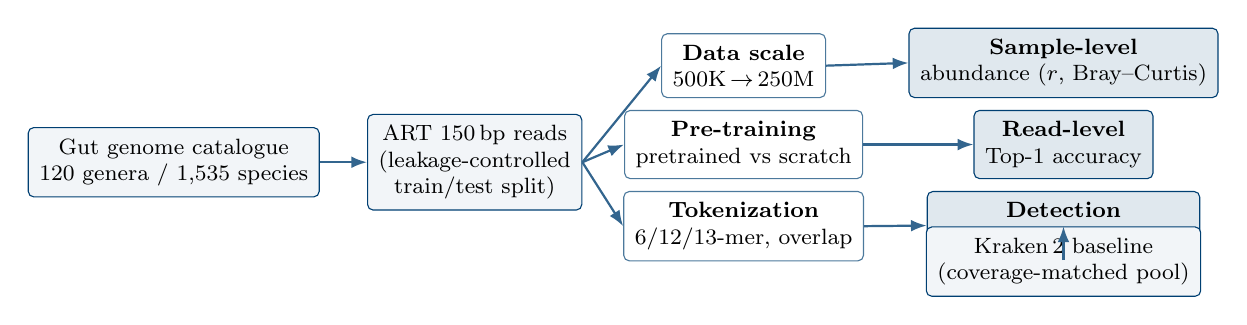
\begin{tikzpicture}[
    font=\footnotesize,
    node distance=6mm,
    box/.style={draw=bibblue,rounded corners=2pt,align=center,
                inner sep=4pt,fill=bibblue!5},
    axis/.style={draw=bibblue!70,rounded corners=2pt,align=center,
                 inner sep=4pt,fill=white},
    ev/.style={draw=bibblue,rounded corners=2pt,align=center,
               inner sep=4pt,fill=bibblue!12},
    ar/.style={-{Latex[length=2mm]},bibblue!80,thick}
  ]
  \node[box] (genomes) {Gut genome catalogue\\120 genera / 1{,}535 species};
  \node[box,right=of genomes] (reads) {ART 150\,bp reads\\(leakage-controlled\\train/test split)};
  \draw[ar] (genomes) -- (reads);

  % ablation axes
  \node[axis,above right=2mm and 10mm of reads] (a1) {\textbf{Data scale}\\500K\,$\to$\,250M};
  \node[axis,below=1.5mm of a1] (a2) {\textbf{Pre-training}\\pretrained vs scratch};
  \node[axis,below=1.5mm of a2] (a3) {\textbf{Tokenization}\\6/12/13-mer, overlap};
  \draw[ar] (reads.east) -- (a1.west);
  \draw[ar] (reads.east) -- (a2.west);
  \draw[ar] (reads.east) -- (a3.west);

  % evaluation
  \node[ev,right=14mm of a2] (e1) {\textbf{Read-level}\\Top-1 accuracy};
  \node[ev,above=1.5mm of e1] (e0) {\textbf{Sample-level}\\abundance ($r$, Bray--Curtis)};
  \node[ev,below=1.5mm of e1] (e2) {\textbf{Detection}\\ROC, sens.\ @ 95\% spec.};
  \draw[ar] (a1.east) -- (e0.west);
  \draw[ar] (a2.east) -- (e1.west);
  \draw[ar] (a3.east) -- (e2.west);

  \node[box,below=6mm of e1] (kraken) {Kraken\,2 baseline\\(coverage-matched pool)};
  \draw[ar] (e2.south) -- (kraken.north);
\end{tikzpicture}%
}
\caption{\textbf{Benchmark design.} Reads are simulated from a leakage-controlled
gut-genome catalogue. Three design axes (data scale, pre-training, tokenization)
are each varied one at a time while the others are held fixed, and every model
is scored at three evaluation levels---read-level accuracy, sample-level
abundance, and binary detection---against a coverage-matched Kraken\,2 baseline.}
\label{fig:design}
\end{figure*}

\section{Data scaling and the saturation effect}
\label{sec:scaling}

We first ask how far data scale alone can carry a fixed pre-trained backbone.
Holding the NT-v2 architecture, LoRA configuration, and 6-mer tokenization
fixed, we increase the training set from 500K to 250M reads
(Figure~\ref{fig:scaling}). Genus Top-1 accuracy (120 classes, with
reverse-complement test-time augmentation) rises steeply at first---55.29\% at
500K, 63.05\% at 5M ($+7.76$ percentage points per 10$\times$), 67.07\% at
50M---then flattens: extending to 250M yields only 67.29\% ($+0.22$ pp for a
further 5$\times$). Over this same range, architectural and training-technique
variations produce at most $\pm0.5$ pp, so within the fixed NT-v2 framework
data volume is the dominant controllable factor, but only up to $\sim$50M reads.

Two observations show this is a ceiling of the representation, not of the data.
First, the underlying unique-read counts (50M $\rightarrow$ 17.8M unique; 250M
$\rightarrow$ 41.9M unique) confirm that most of the extra reads are repeats, so
the marginal information added past 50M is modest---but not zero, and certainly
not enough to explain complete saturation. Second, and decisively, the same
data does \emph{not} saturate a different tokenizer: an overlapping-13-mer
MetaTransformer trained on the identical $50\text{M}\!\rightarrow\!250\text{M}$
reads improves from 87.5\% to 98.7\% genus Top-1 over exactly the range where
NT-v2 is flat (Section~\ref{sec:decomp}). The saturation is therefore a
property of the 6-mer tokenizer, not of the training corpus.

Reverse-complement test-time augmentation---averaging predictions over a read
and its reverse complement---gives a small but consistent improvement of
$+0.1$ to $+1.5$ pp across all settings (Figure~\ref{fig:rctta}), reflecting the
strand symmetry of the underlying biology
\citep{Zhou2022rc,Brown2021rc,Ma2025rc}; we apply it to all NT-v2 numbers.

\begin{figure}[t]
\centering
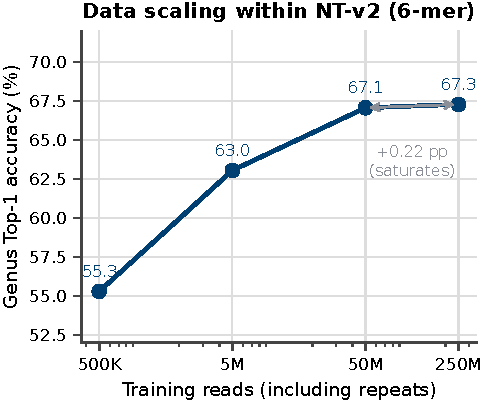
\includegraphics[width=\columnwidth]{data_scaling.pdf}
\caption{\textbf{Data scaling within a fixed NT-v2 backbone.} Genus Top-1
accuracy as a function of training-read count (log scale; $x$-axis counts reads
including repeats). Accuracy climbs from 500K to 50M then saturates: the
$5\times$ step from 50M to 250M adds only $+0.22$ pp. The plateau is set by the
non-overlapping 6-mer tokenizer, not by data availability
(cf.\ Section~\ref{sec:decomp}).}
\label{fig:scaling}
\end{figure}

\begin{figure}[t]
\centering
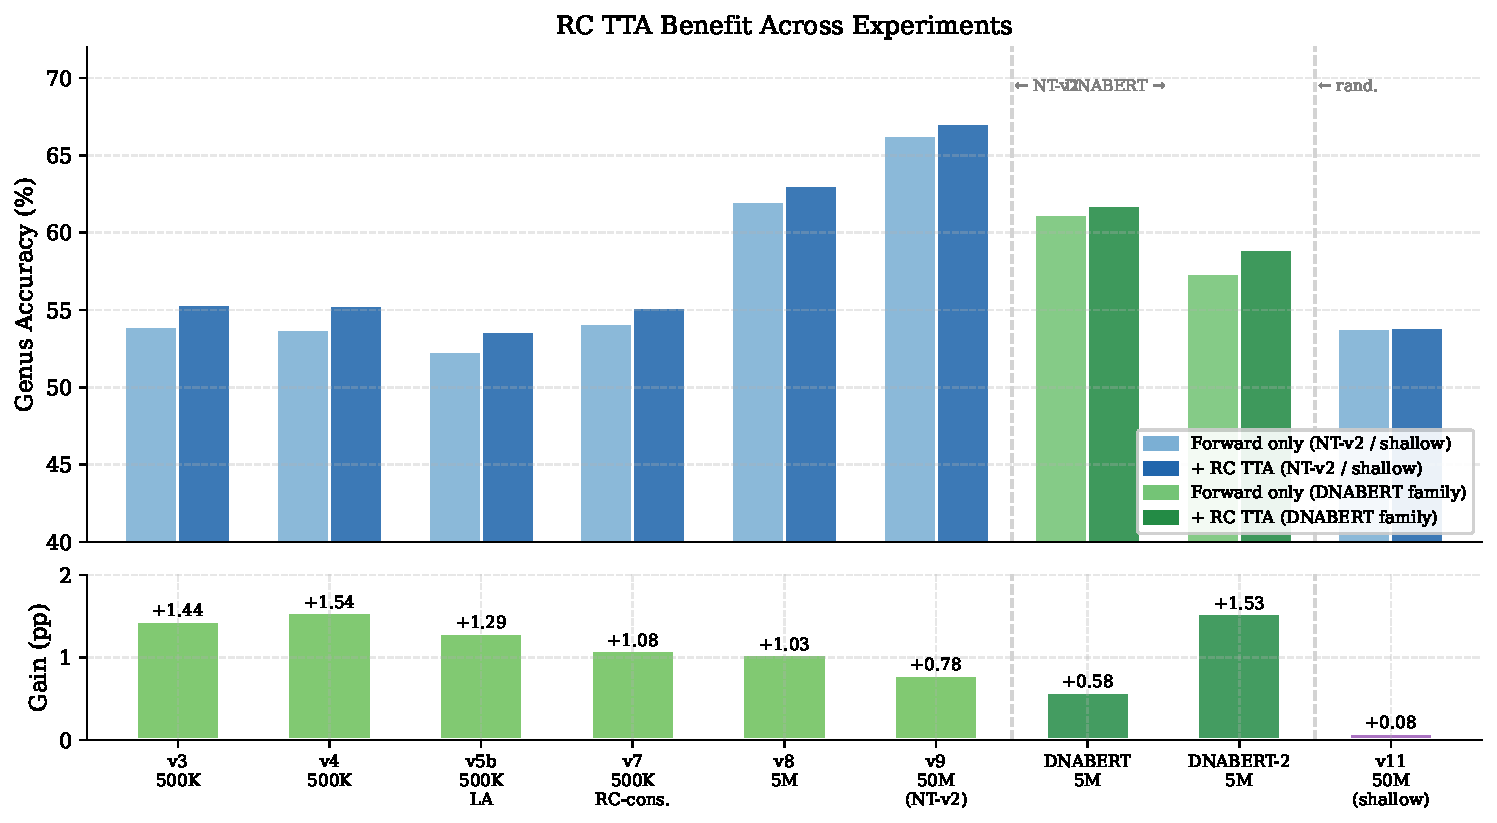
\includegraphics[width=\columnwidth]{rc_tta_benefit.pdf}
\caption{\textbf{Reverse-complement test-time augmentation.} Averaging over a
read and its reverse complement yields a consistent $+0.1$ to $+1.5$ pp gain
across settings, exploiting strand symmetry at no training cost.}
\label{fig:rctta}
\end{figure}

\paragraph{Class balancing is counterproductive for real abundance.}
Because the label space is long-tailed, one might rebalance classes to help
rare taxa. At a fixed 17.6M-read budget, we compared species-balanced and
genus-balanced sampling (varying only the balancing axis). Genus-balancing
raises the flat, per-genus-averaged accuracy from 33.1\% to 43.5\%
($+10$ pp on the macro metric), but it \emph{lowers} per-read accuracy from
60.4\% to 37.2\% ($-23$ pp) and degrades sample-level abundance fidelity from
Pearson $r=0.993$ to $r=0.862$. The $\sim$42--43\% flat ceiling persists even
under balancing, indicating that most of the difficulty is intrinsic to
150\,bp reads rather than a fixable imbalance artefact. For applications that
report community composition, aggressive class-balancing therefore does more
harm than good---a concrete recommendation we return to in
Section~\ref{sec:recommendations}.

\section{Pre-training versus tokenization}
\label{sec:decomp}

We now separate the two factors that a data-scaling curve alone cannot
distinguish: the value of pre-training and the value of tokenization. The
experiment is designed so that each can be isolated by changing exactly one
variable.

\subsection{Pre-training, at fixed tokenization, helps}

Holding tokenization fixed at non-overlapping 6-mer and data fixed at 50M
reads, we replace the pre-trained 29-layer NT-v2 backbone with a single-layer
randomly initialized transformer. The pre-trained backbone reaches 67.07\%
genus Top-1 versus 53.88\% for the random-initialized model---a $+13.19$ pp
pre-training advantage (Figure~\ref{fig:ablation}). Pre-training on genomic
sequence thus provides a real, transferable benefit for this task even though
the pre-training corpus is not microbial. This is the strongest case for GFMs
in metagenomics: the representation learned during pre-training is worth more
than 13 accuracy points that no amount of extra 6-mer data recovers.

\subsection{Tokenization, at fixed capacity, helps more}

Holding data fixed at 50M reads and training \emph{from scratch} (no
pre-training on either side), we vary only the tokenizer within the
MetaTransformer architecture. The effect dwarfs pre-training
(Table~\ref{tab:tok}): overlapping 13-mer reaches 87.42\% genus Top-1 while
overlapping 6-mer reaches only 48.87\% and non-overlapping 6-mer 47.00\%.
The overlapping-13-mer model trained from scratch (87.42\%) outperforms the
498M-parameter pre-trained NT-v2 with 6-mer tokenization (67.07\%) by
$+20.35$ pp on identical data. In other words, changing the tokenizer buys more
than changing from a shallow random network to a large pre-trained one. NT-v2's
non-overlapping 6-mer tokenization is the principal structural limitation of
the GFM approach here---not backbone capacity and not the adaptation strategy.

\begin{table*}[t]
\centering
\caption{\textbf{Tokenization governs both the ceiling and the ability to
scale.} Genus Top-1 accuracy (120 classes). MetaTransformer (MT) rows are
trained from scratch; NT-v2 is pre-trained. Only overlapping 13-mer reaches the
high-80s/90s and continues to improve from 50M to 250M reads, whereas 6-mer
representations plateau at 45--67\% regardless of pre-training or data.}
\label{tab:tok}
\begin{tabular*}{\textwidth}{@{\extracolsep{\fill}}lllcc@{}}
\toprule
Tokenizer & Overlap & Model & 50M & 250M \\
\midrule
13-mer & stride 1 (overlap)      & MT (scratch)      & 87.42\% & \textbf{98.7\%} \\
12-mer & stride 1 (overlap)      & MT (scratch)      & 78.83\% & --- \\
6-mer  & stride 1 (overlap)      & MT (scratch)      & 48.87\% & 50.6\% \\
6-mer  & non-overlap (stride 6)  & MT (scratch)      & 47.00\% & 45.0\% \\
6-mer  & non-overlap             & NT-v2 (pre-trained)& 67.07\% & 67.29\% \\
\botrule
\end{tabular*}
\end{table*}

Critically, tokenization also governs \emph{scalability}. As data grows from
50M to 250M, the overlapping-13-mer model improves by $+11$ pp
($87.5\%\!\rightarrow\!98.7\%$) while the 6-mer NT-v2 is flat ($+0.22$ pp;
Section~\ref{sec:scaling}). A tokenizer that preserves enough local signal both
raises the ceiling and keeps the model in the regime where more data helps.

\begin{figure}[t]
\centering
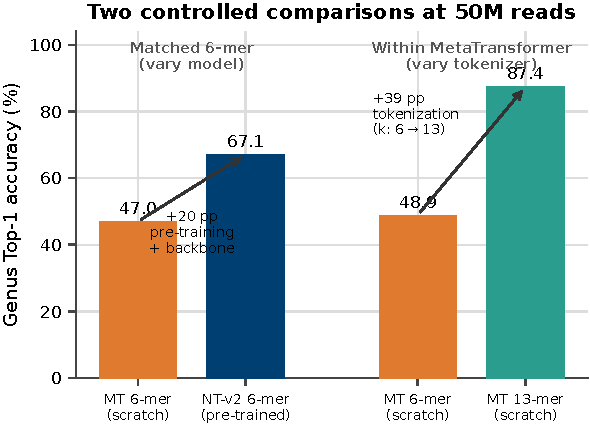
\includegraphics[width=\columnwidth]{backbone_ablation.pdf}
\caption{\textbf{Decomposing the sources of accuracy on a common 50M-read
baseline.} Left to right: a randomly initialized shallow 6-mer model; the
pre-trained NT-v2 6-mer model ($+13.2$ pp from pre-training, at fixed
tokenization); and an overlapping-13-mer model trained from scratch
($+20.4$ pp over pre-trained NT-v2, from tokenization alone). Tokenization is
the larger lever.}
\label{fig:ablation}
\end{figure}

\subsection{The ceiling is representational, not one of capacity or optimization}

A natural objection is that the 6-mer model is simply under-trained or
under-parameterized. The training-fit numbers refute this. The NT-v2 6-mer
model cannot even \emph{fit} the training set past $\sim$66\% (250M warm-start:
65.8\% train, 66.6\% validation---train and validation almost equal), whereas
the 13-mer model fits training to 98.9\% and validates at 97.5\%. When a model
cannot memorize the training data, the bottleneck is the input representation,
not capacity, data, or generalization: the non-overlapping 6-mer tokens simply
do not carry enough separable signal for a 150\,bp read.

\begin{figure}[t]
\centering
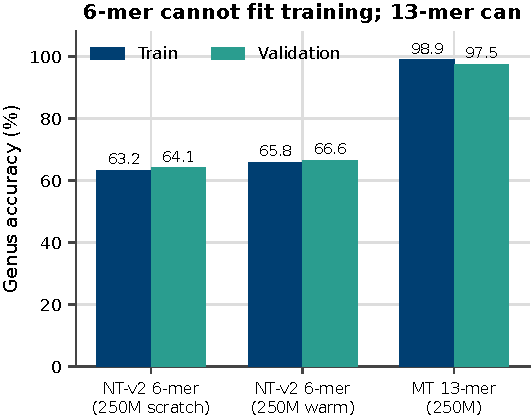
\includegraphics[width=\columnwidth]{train_fit.pdf}
\caption{\textbf{The ceiling is representational, not one of capacity.} Training
versus validation genus accuracy. The 6-mer model cannot fit the training set
past $\sim$66\% (train $\approx$ validation), whereas the overlapping-13-mer
model fits to 98.9\%. A model that cannot memorize its training data is limited
by its input representation, not by capacity or data.}
\label{fig:trainfit}
\end{figure}

\subsection{Is the 13-mer result just closed-set lookup?}
\label{sec:lookup}

The obvious worry about a 98.7\% number is that a 13-mer model is performing
disguised exact-match lookup against the reference---i.e.\ memorizing rather
than generalizing. We tested this directly by building non-neural $k$-mer
classifiers on the same 50M-read reference and the same test pool. A
Kraken-style unique-key lookup achieves only 0.72\% (because $k=13$ is
\emph{not} genus-unique: the $4^{13}=67.1$M 13-mer space is saturated by the
1{,}535 genomes, so test 13-mers are almost all ``seen'' but only $\sim$0.4\%
map to a single genus). A dominant-genus majority vote reaches 35.3\%, and a
full multinomial $k$-mer naive Bayes---using $P(k\text{-mer}\mid\text{genus})$
without any neural network---reaches 74.9\%. The MT 13-mer network adds a
further $+13$ pp over naive Bayes (87.5\%), capturing co-occurrence structure
beyond the naive-Bayes independence assumption. The mechanism is therefore
learned high-dimensional composition, \emph{not} exact-match lookup
(Figure~\ref{fig:kmer}).

\begin{figure}[t]
\centering
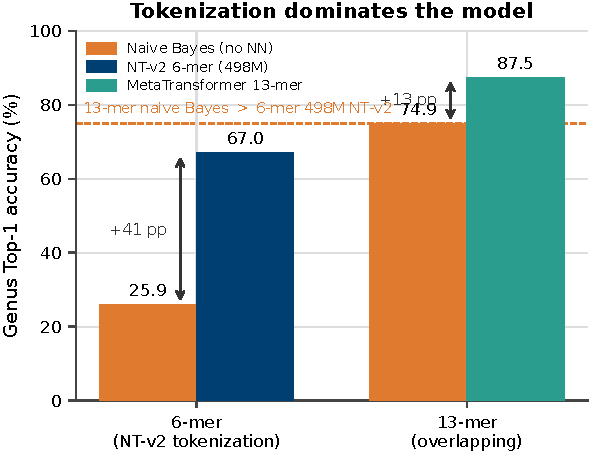
\includegraphics[width=\columnwidth]{kmer_baselines.pdf}
\caption{\textbf{Composition, not lookup.} Genus Top-1 accuracy of non-neural
$k$-mer classifiers on the same 50M-read reference and test pool, versus the
neural models. Exact-match unique-key lookup fails (0.7\%) because $k=13$ is not
genus-unique; a parameter-free multinomial 13-mer naive Bayes already reaches
74.9\%, \emph{exceeding} the 498M-parameter pre-trained NT-v2 (67\%). The neural
13-mer model adds a further $+13$ pp over naive Bayes.}
\label{fig:kmer}
\end{figure}

This analysis also delivers the paper's sharpest single comparison: a
parameter-free 13-mer naive Bayes (74.9\%) \emph{beats} the 498M-parameter
pre-trained NT-v2 with 6-mer tokenization (67\%). Representation ($k$-mer
length) is more decisive than model capacity or pre-training. We are explicit
about the accompanying caveat: because the reference genomes are nearly
completely covered by the test organisms, the 98.7\% figure characterizes
\emph{closed-set} classification against known genomes; novel-genome
generalization is a separate question that we flag as the primary limitation
(Section~\ref{sec:limitations}).

\section{Read-level accuracy versus sample-level utility}
\label{sec:sample}

Read-level accuracy measures raw discriminative power, but practitioners
usually care about the community profile: the relative abundance of each taxon
in a sample. These two quantities can diverge, because independent per-read
errors partially cancel when aggregated. We therefore evaluate every model at
the sample level---relative-abundance estimation and binary detection---and
compare against Kraken\,2 on a database-coverage-matched pool.

\subsection{Per-read errors largely cancel in abundance estimates}

On synthetic species-balanced samples (9 samples $\times$ 10K reads from the
natural-distribution pool), a 67\%-accurate read classifier yields a
genus relative-abundance Pearson $r=0.993$ and Bray--Curtis dissimilarity
$0.098$ (Table~\ref{tab:sample}, Figure~\ref{fig:abund}). The overlapping-13-mer
model, with far higher read accuracy, reaches $r\!\approx\!1.000$. The ranking
by sample-level fidelity follows the ranking by read accuracy, but even the
mid-accuracy model is highly usable for abundance because misclassifications
are not systematically biased toward any one genus and thus average out. We
report $r$ as a range rather than a single value, because it is pool-dependent
(e.g.\ NT-v2 gives $r=0.928$ on the harder leftover pool); the genus-balanced
model, consistent with Section~\ref{sec:scaling}, is the clear outlier at
$r=0.862$.

We deliberately distinguish three levels of sample-level evaluation, of
increasing difficulty: (i) fixed-composition random partitions of a common read
pool (used here); (ii) sparse synthetic communities with variable composition;
and (iii) real or mock communities with authentic error profiles and incomplete
database coverage. The present results establish (i)---a stability test under a
fixed expected composition---and should not be read as evidence for (iii): they
show that per-read errors cancel when the community is held fixed, not that a
6-mer model can profile an arbitrary real sample. We therefore probe (iii) later
in this section on a real mock community (Section~\ref{sec:mock}); that probe is
preliminary, and a fuller multi-community evaluation remains required before
deployment (Section~\ref{sec:limitations}).

\begin{table}[t]
\centering
\caption{\textbf{Sample-level genus abundance} on the natural-distribution
pool (9$\times$10K reads). Higher read accuracy tracks better abundance
fidelity, but even a 67\%-accurate model attains $r=0.99$. Genus-balancing
(bottom row) is counterproductive.}
\label{tab:sample}
\begin{tabular*}{\columnwidth}{@{\extracolsep{\fill}}lccc@{}}
\toprule
Model & Read acc.\ & Pearson $r$ & Bray--Curtis \\
\midrule
MT 13-mer (250M)         & 98.7\% & 1.000 & 0.005 \\
MT 13-mer (50M)          & 87.4\% & 0.999 & 0.032 \\
NT-v2 6-mer (50M)        & 67.1\% & 0.993 & 0.098 \\
NT-v2 6-mer (250M warm)  & 67.3\% & 0.993 & 0.098 \\
MT 6-mer (scratch)       & 48.9\% & 0.989 & 0.171 \\
NT-v2 genus-balanced     & 37.2\% & 0.862 & 0.420 \\
\botrule
\end{tabular*}
\end{table}

\begin{figure*}[t]
\centering
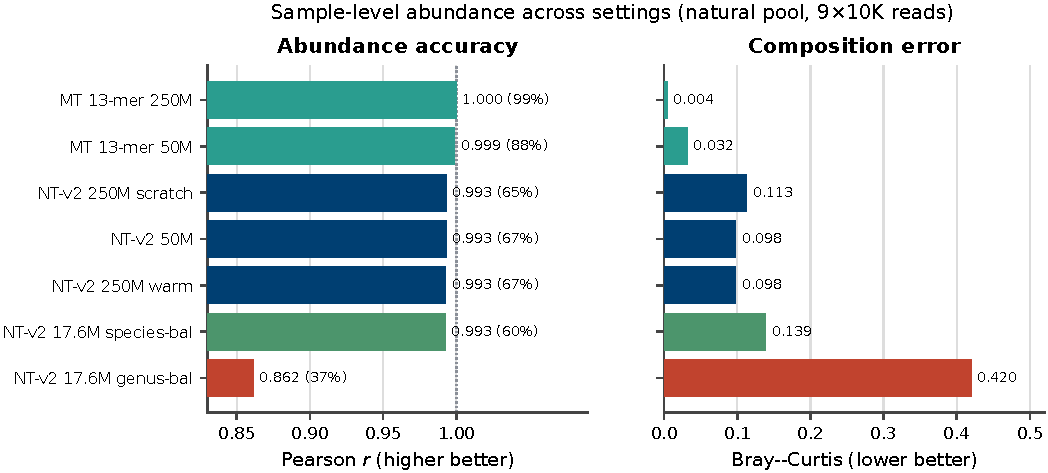
\includegraphics[width=\textwidth]{cross_setting_comparison.pdf}
\caption{\textbf{Sample-level abundance fidelity across settings} on the
natural-distribution pool (9$\times$10K reads), sorted by Pearson $r$; read-level
accuracy is shown in parentheses. Abundance correlation stays high
($r\approx0.99$) down to $\sim$60\% read accuracy because independent per-read
errors cancel in aggregate. Genus-balancing is the clear outlier
($r=0.86$, Bray--Curtis $0.42$): it skews predictions toward rare genera and
distorts the natural composition.}
\label{fig:abund}
\end{figure*}

\subsection{Comparison with Kraken\,2: abundance versus detection}

On the coverage-matched genus pool (85{,}819 reads whose source species are in
the Kraken\,2 database), we separate two questions---\emph{how much} (abundance)
and \emph{whether present} (detection)---and compare the neural models against
Kraken\,2 both as raw report counts and with Bracken re-estimation
(Table~\ref{tab:kraken}, Figure~\ref{fig:kraken}). For abundance, raw Kraken\,2
counts give only Pearson $r=0.823$: Kraken\,2 leaves $\sim$30\% of reads
unclassified and, because that abstention is spread across taxa, it uniformly
deflates predicted abundances. This is a fixable artefact, not a fundamental
limit---Bracken \citep{Lu2017}, which re-estimates abundance from the same
Kraken\,2 report, raises genus abundance to $r=0.997$ (Bray--Curtis $0.060$) on
the same reads and database. Bracken therefore reaches the same near-perfect
range as the neural models (MT 13-mer $r=0.999$, NT-v2 $r=0.992$):
\textbf{the neural models have no sample-level abundance advantage over a
properly configured classical pipeline.} (Bracken redistributes the whole report and cannot be restricted per
read to the in-database subset; on the full 100K sample raw Kraken\,2 is
$r=0.845$, so this is a like-for-like comparison.) For detection, Kraken\,2---and
Bracken, which inherits its classifications---dominates (ROC AUC 0.966, 93.5\%
sensitivity at 95\% specificity), far above the 6-mer neural detectors (NT-v2
AUC 0.681, 17.5\%), with the overlapping-13-mer model in between (AUC 0.905,
66.5\%). On in-database data, then, the classical Kraken\,2$+$Bracken pipeline is
the stronger tool for \emph{both} abundance and detection; the neural models'
genuine advantages lie elsewhere---higher read-level accuracy under a good
tokenizer (MT 13-mer 94.9\% vs Kraken\,2 77.7\%) and graceful degradation
outside the reference database (below, where Kraken\,2 scores 0\% on 219
out-of-database species).

\begin{table*}[t]
\centering
\caption{\textbf{Genus-level, coverage-matched comparison with Kraken\,2}
(85{,}819 in-database reads). Raw Kraken\,2 abundance is deflated by its
$\sim$30\% abstention ($r=0.823$); re-estimating with Bracken raises Kraken\,2
genus abundance to $r=0.997$ (main text), on par with the best neural model, so
the neural advantage on abundance disappears against the proper pipeline.
Kraken\,2 also dominates detection. Sens@95 = sensitivity at 95\% specificity.}
\label{tab:kraken}
\begin{tabular*}{\textwidth}{@{\extracolsep{\fill}}lccccc@{}}
\toprule
Model & Read acc.\ & Pearson $r$ & Bray--Curtis & ROC AUC & Sens@95 \\
\midrule
MT 13-mer            & 94.9\% & \textbf{0.999} & 0.029 & 0.905 & 66.5\% \\
NT-v2 6-mer          & 68.9\% & 0.992 & 0.116 & 0.681 & 17.5\% \\
Kraken\,2 ($k{=}35$) & 77.7\% & 0.823 & 0.126 & \textbf{0.966} & \textbf{93.5\%} \\
MT 6-mer             & 51.5\% & 0.983 & 0.177 & 0.576 & 9.2\% \\
\botrule
\end{tabular*}
\end{table*}

\begin{figure}[t]
\centering
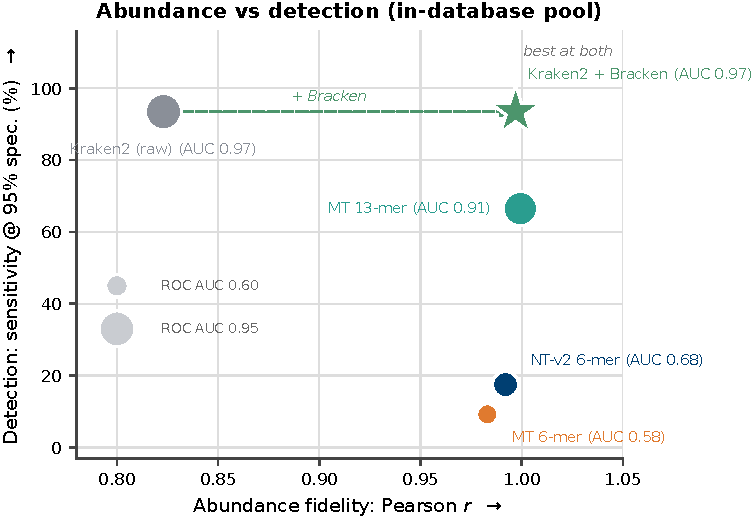
\includegraphics[width=\columnwidth]{tradeoff_abundance_detection.pdf}
\caption{\textbf{Abundance versus detection on the in-database pool}
(coverage-matched, 85{,}819 reads); marker area scales with ROC AUC. The neural
models reach high abundance fidelity (Pearson $r$) but weak detection
sensitivity. Raw Kraken\,2 is the opposite (strong detector, deflated abundance),
but \emph{Bracken re-estimation moves the classical pipeline to the top-right}
($r=0.997$, sensitivity 93.5\%)---best at both. On in-database data the neural
models therefore hold no advantage here; their value lies off this plot, in
read-level accuracy and out-of-database robustness (Section~\ref{sec:sample}).}
\label{fig:kraken}
\end{figure}

\subsection{Species level reveals the same tokenizer bottleneck}

At the species level (1{,}535 classes) the gap widens in Kraken\,2's favour on
the coverage-matched pool (77.2\% read accuracy, $r=0.847$), because exact long
$k$-mers resolve fine taxonomy that 6-mer neural models cannot: a flat NT-v2
6-mer species classifier reaches only 17.6\% Top-1, versus $\sim$50\% for the
overlapping-13-mer model. The natural remedy is a hierarchical pipeline---route a
read to its genus, then to a species within that genus---but this only helps with
a near-perfect router. Under \emph{oracle} genus routing, per-genus classifiers
lift species Top-1 to 29.5\%; with a \emph{realistic} learned router (genus
accuracy $\sim$66\%, itself the 6-mer ceiling of Section~\ref{sec:decomp}) the
same pipeline falls to 15.6\%---at or below the flat model. The bottleneck is
therefore the genus router, not the per-genus heads (oracle routing makes
genus-level accuracy $1.00$ by construction), so the 6-mer genus ceiling
propagates directly into species performance. Overlapping long-$k$ tokenization
is thus the shared fix for both genus routing and intra-genus separation; adding
a sub-genus split \emph{without} a better representation instead hurts (a
negative result; Supplementary). Conversely, Kraken\,2's dependence
on database coverage is a real liability---on 219 species outside its custom
database it scores 0\% while the neural models retain non-zero posterior mass,
the flip side of the abstention behaviour above.

Finally, the abstention-free behaviour of neural models has a cost for rare
taxa: a genuinely absent genus still receives a small number of spurious reads
(on the order of $\sim$0.28\% of a sample), setting a noise floor below which
detection is unreliable. This noise floor has a clean interpretation and
motivates the calibrated-threshold recommendation in
Section~\ref{sec:recommendations}.

\subsection{A real mock community: the in-database dominance does not transfer}
\label{sec:mock}

All comparisons so far use simulated reads. As a first check on real data, we
ran the trained genus classifiers and the Kraken\,2$+$Bracken pipeline
(inference only) on two Illumina WGS replicates of the ZymoBIOMICS Gut
Microbiome Standard (D6331; SRR33710519 and SRR33710518; 3M R1 reads each,
median 135\,bp). The vendor genomic-DNA percentages are the sample-level ground
truth. Of the 21 mock taxa, 11 genera (81.5\% of the community) fall within our
120 training genera; the remainder are out-of-set (dominated by
\emph{Escherichia} at 14\%, absent from the 120 genera), an unavoidable ceiling
for every method. Metrics are means over the two replicates
(Table~\ref{tab:mock}); per-replicate values and per-genus residuals are in the
Supplementary Material.

Two things change relative to the simulated in-database pool. First,
\emph{every} method's genus-abundance correlation collapses from
$r\approx0.99$--$0.997$ to $r\approx0.41$--$0.58$ (Spearman
$\rho\approx0.34$--$0.57$): the closed-set numbers do not transfer to real
reads. With only 11 in-set genera as points, bootstrap 95\% intervals on Pearson
$r$ are wide and overlapping, so we do \emph{not} rank methods by $r$.
Restricting to the nine genera with expected abundance $\ge$1\% raises all three
correlations into a tighter band ($r\approx0.57$--$0.62$), confirming that the
headline gap is driven partly by near-zero taxa and a few large residuals rather
than a stable method ordering. Second, the classical pipeline's simulated
dominance evaporates. Kraken\,2 classifies only $\sim$44\% of the real reads
($\sim$56\% unclassified, versus $\sim$30\% on simulation); even after Bracken,
detection sensitivity among genera expected at $\ge$1\% is 55.6\%---below the
neural models (NT-v2 83.3\%, MT 77.8\%)---and Bray--Curtis error is the worst of
the three (0.434), inflated by over-estimating \emph{Veillonella}. Always-labelling
neural models are competitive on composition error (MT best at 0.353; NT-v2
0.384).

Shared failure modes appear in both replicates and both neural models:
\emph{Roseburia} (17\% expected after in-set renormalization) is nearly missed
($\sim$0.5\%), while \emph{Clostridium} absorbs substantial mass
($\sim$12--18\% predicted vs $\sim$0 expected)---partly because
\emph{Clostridioides difficile} (1.5\% of the mock; out-of-set under current
taxonomy) may map into the training \emph{Clostridium} label if older names
were used. Out-of-set \emph{Escherichia} leaks into neighbouring
Enterobacteriaceae false positives. These patterns mix real-error behaviour with
strain/taxonomy mismatch, so the probe is not a pure sequencing-artefact test.

\begin{table}[t]
\centering
\caption{\textbf{Real mock community} (ZymoBIOMICS D6331; mean of two
replicates; 11 in-set genera, 18.5\% out-of-set). Pearson $r$ intervals overlap
heavily ($n{=}11$); Sens.\ = detection among genera with expected
abundance $\ge$1\% (predicted fraction $\ge$1\%). No method wins on all axes.}
\label{tab:mock}
\begin{tabular*}{\columnwidth}{@{\extracolsep{\fill}}lcccc@{}}
\toprule
Method & Pearson $r$ & Bray--Curtis & Sens.\ @1\% & Reads clf.\ \\
\midrule
Kraken\,2$+$Bracken & 0.578 & 0.434 & 55.6\% & 43.9\% \\
MT 13-mer           & 0.538 & 0.353 & 77.8\% & 100\% \\
NT-v2 6-mer         & 0.412 & 0.384 & 83.3\% & 100\% \\
\botrule
\end{tabular*}
\end{table}

This two-replicate probe (11 in-set genera, 135\,bp reads) remains preliminary
rather than a definitive multi-community benchmark. It does make one point
cleanly: the classical pipeline's crushing in-database advantage
(Section~\ref{sec:sample}) is a property of simulated, fully-covered data, not
of real communities---on real reads the neural models are competitive, and the
binding open problem for \emph{all} methods is the large gap between closed-set
and real-world accuracy. A fuller evaluation across additional communities,
matched read lengths, and further baselines is the priority follow-up
(Section~\ref{sec:limitations}).

\section{Practical recommendations}
\label{sec:recommendations}

The controlled results above translate into concrete guidance. We separate
recommendations for practitioners choosing or applying a tool today from
recommendations for those designing the next generation of models.

\subsection{For practitioners}

\begin{table*}[t]
\centering
\caption{\textbf{Use-case-specific recommendations.} ``long-$k$ model'' denotes
an overlapping long-$k$-mer neural classifier; ``6-mer GFM'' denotes a
pre-trained NT-v2-style model with non-overlapping 6-mer tokenization.}
\label{tab:reco}
\begin{tabularx}{\textwidth}{@{}p{0.30\textwidth}X@{}}
\toprule
Use case & Recommendation \\
\midrule
Read-level genus classification &
Prefer an overlapping long-$k$ model (87\% vs 67\%); a 6-mer GFM is a distant
second. \\[2pt]
Sample-level abundance (composition) &
A 67\%-accurate model is often sufficient ($r=0.99$) and can beat Kraken\,2 by
avoiding abstention bias---but validate for systematic bias on your community. \\[2pt]
Presence/absence detection, esp.\ low-abundance taxa &
Use Kraken\,2 (or another exact-$k$-mer tool); current 6-mer neural detectors
are weak. Apply a calibrated abundance threshold above the $\sim$0.3\% noise
floor. \\[2pt]
Species-level classification &
6-mer GFMs are insufficient; use a long-$k$ tokenizer or a hierarchical router,
or an exact-$k$-mer tool when the target is in-database. \\[2pt]
Handling class imbalance &
Do \emph{not} aggressively genus-balance if you report abundance: it lifts macro
metrics but harms per-read accuracy and abundance fidelity ($r\!:0.99\!\to\!0.86$). \\[2pt]
Choosing a GFM &
Do not select on backbone size alone; the tokenizer decides whether taxonomic
signal survives. Ask what $k$ and what stride the model uses. \\
\botrule
\end{tabularx}
\end{table*}

\subsection{For model builders}

The single highest-leverage design choice is tokenization. Future microbial
foundation models intended for short-read taxonomy should be \emph{pre-trained}
with overlapping long-$k$ tokenization (e.g.\ 12--13-mers), combining the
discriminative power that overlapping long $k$-mers provide with the
representational quality that pre-training adds---the two independent gains we
quantified ($+20$ pp from tokenization, $+13$ pp from pre-training). Because a
naive long-$k$ vocabulary is enormous (a 13-mer vocabulary implies a
multi-billion-parameter embedding table; the ``$\sim$5M-parameter''
MetaTransformer figure counts only the encoder and understates true cost),
practical realizations will need vocabulary factorization, hashing, or hybrid
tokenization---an open engineering problem we regard as the key next step.
Pre-training corpora should draw on the hundreds of thousands of microbial
genomes now catalogued \citep{Parks2022,Almeida2019} rather than
eukaryote-dominated data.

\section{Limitations and future directions}
\label{sec:limitations}

\paragraph{Closed-set evaluation.}
The headline 98.7\% and $r\!\approx\!1$ figures characterize classification
against genomes that are present in the reference. Because our test organisms
are drawn from the same catalogue used to build the training reference, these
numbers measure closed-set performance, not novel-genome generalization. We
showed the mechanism is learned composition rather than exact-match lookup
(Section~\ref{sec:lookup}), but the more demanding question---how accuracy
transfers to genomes of the same genera that were \emph{withheld} from
training---is the single most important open item. An out-of-genome
generalization experiment (holding out a subset of each genus's genomes from
training) is the natural next step and is required before the tokenization
advantage can be claimed for real-world discovery settings.

\paragraph{Simulated reads.}
Reads were generated with ART \citep{Huang2012}. Simulation may favour
alignment- and $k$-mer-based methods with structurally clean error models, and
does not capture all real sequencing artefacts. Our probe on a real mock
community (ZymoBIOMICS D6331, two Illumina replicates; Section~\ref{sec:mock}),
with a matched Kraken\,2$+$Bracken baseline, shows all methods dropping to
$r\approx0.41$--$0.58$ with overlapping uncertainty ($n{=}11$ in-set genera) and
Kraken\,2 abstaining on $\sim$56\% of reads---a substantial closed-set-to-real
gap. Replicate-to-replicate agreement is tight, but the community is still a
single standard (11 in-set genera, 135\,bp reads); a fuller evaluation across
multiple communities, matched read lengths, and additional baselines
(e.g.\ Centrifuge) remains the priority follow-up.

\paragraph{Baseline breadth.}
We compare against Kraken\,2 both as raw report counts and with Bracken
\citep{Lu2017} abundance re-estimation (Section~\ref{sec:sample}); Bracken is the
appropriate abundance baseline and is strong ($r=0.997$ on the simulated
in-database pool). A fuller benchmark should also add Centrifuge
\citep{Kim2016} or other classifiers so that the neural models are measured
against the broadest set of production pipelines.

\paragraph{Single read length and evaluation asymmetry.}
Simulated experiments use 150\,bp reads; the real mock probe uses median
135\,bp reads from the same Illumina run. Generalization to other read lengths
(75/250\,bp) is untested. We also note a metric asymmetry in the current
results---NT-v2 numbers use reverse-complement test-time augmentation while
MetaTransformer numbers are forward-only---which slightly understates the
MetaTransformer models (RC-TTA adds $\sim$0.7 pp); harmonizing this is
straightforward and does not affect any qualitative conclusion.

\paragraph{Outlook.}
The consistent thread is that input representation, not model scale, is the
binding constraint for short-read taxonomy with foundation models. The most
promising direction is a microbial foundation model pre-trained with
overlapping long-$k$ tokenization and an efficient large-vocabulary embedding,
evaluated from the outset with the leakage control, out-of-genome splits, and
dual read/sample metrics used here.

%=======================================================================
%  ENDMATTER STATEMENTS  (required by Briefings in Bioinformatics)
%  Section titles follow the OUP authoring-template conventions.
%=======================================================================
\section{Conflicts of interest}
The authors declare that they have no competing interests.

\section{Funding}
[Funding sources and grant numbers to be inserted.] Computation was supported by
the National Center for High-performance Computing (NCHC), Taiwan.

\section{Data availability}
The reference genome catalogue is available from its original source
\citep{Almeida2019}. Simulated reads, trained model checkpoints, per-read
prediction files, and the sample-level evaluation outputs are deposited at
[repository name] at [URL/DOI to be inserted on acceptance]. The read-simulation,
training, and evaluation code is available at
\url{https://github.com/m2lab-ntu/gfm-classifier}.

\section{Code availability}
All training, inference, and evaluation scripts, together with model
configuration files and the exact training commands used for each experiment,
are provided in the repository above and summarized in the Supplementary
Material to enable reproduction.

\section{Author contributions statement}
Using the CRediT taxonomy (authors identified by initials):
X.X. conceived and designed the study, implemented the software, ran the
experiments, analysed the results, and wrote the original draft;
Y.Y. supervised the work, acquired resources and funding, and reviewed and
edited the manuscript. All authors read and approved the final manuscript.
% Replace initials and roles with the actual author list before submission.

\section{Acknowledgments}
The authors thank [colleagues/reviewers] for helpful discussions. During the
preparation of this work an AI coding/writing assistant was used to help draft
and edit the manuscript \LaTeX{} and to organize experimental results. All
experimental design, analysis, interpretation, and final scientific claims are
the authors' own; the authors verified all reported numbers against the
underlying results and take full responsibility for the content. No AI tool is
listed as an author.


% Use unsrtnat (numbered, in order of appearance = Vancouver/BIB style).
% NB: do NOT use the bundled oup-plain.bst here -- it emits bare \bibitem{key}
% entries, which makes the class flip natbib back to author-year mode and
% produces empty "[ , ]" citations. unsrtnat writes labelled \bibitem[..]{key}
% so the numeric citations resolve correctly.
\bibliographystyle{unsrtnat}
\bibliography{references}

\end{document}
